\documentclass{ctexart}
% \usepackage{bm}
\usepackage{tikz}

% \usefonttheme[onlymath]{serif}% 数学公式字体设置

\begin{document}


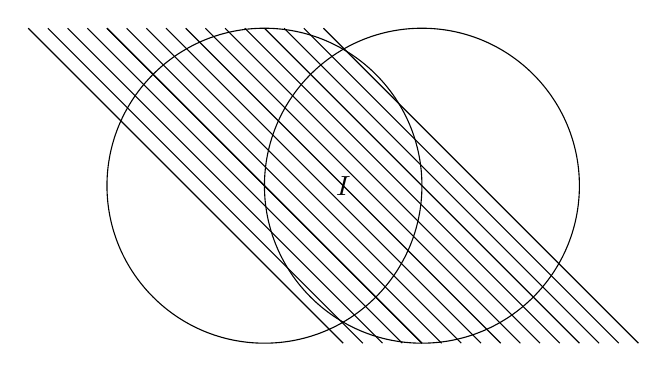
\begin{tikzpicture}
    \draw (0,0) circle (2cm);
    \draw (2,0) circle (2cm);
    % \clip[draw] (0,0) circle (2cm);
    % \clip[draw] (2,0) circle (2cm);
    \foreach \x in {-1,-0.75,-0.5,-0.25,0,0,
        0.25,0.5,0.75,1,1.25,1.5,1.75,2,2.25,2.5,2.75}
    \draw[xshift=\x cm]  (-2,2)--(2,-2);
    \node at (1,0) {$I$};
\end{tikzpicture}

% \raisebox{0pt}[0pt][0pt]{\Large%
% \textbf{Aaaa\raisebox{-0.3ex}{a}%
% \raisebox{-0.7ex}{aa}%
% \raisebox{-1.2ex}{r}%
% \raisebox{-2.2ex}{g}%
% \raisebox{-4.5ex}{h}}}
% he shouted but not even the next
% one in line noticed that something
% terrible had happened to him.

% \flushleft
% \newenvironment{vardesc}[1]{%
% \settowidth{\parindent}{#1:\ }
% \makebox[0pt][r]{#1:\ }}{}
% % \begin{displaymath}
% % a^2+b^2=c^2
% % \end{displaymath}
% \begin{vardesc}{Where}$a$,
%     $b$ -- are adjunct to the right
%     angle of a right-angled triangle.

%     $c$ -- is the hypotenuse of
%     the triangle and feels lonely.
    
%     $d$ -- finally does not show up
%     here at all. Isn’t that puzzling?
% \end{vardesc}

% \tikz \draw[thick,rounded corners=8pt]
% (0,0) -- (0,2) -- (1,3.25) -- (2,2) -- (2,0) -- (0,2) -- (2,2) -- (0,0) -- (2,0);

% xx
% \begin{tikzpicture}
%     \draw[line width=6pt](0, 0)circle(10pt);
% \end{tikzpicture}
% xx

% xx
% \begin{tikzpicture}
%     [baseline=(X.base)]
%     % \draw[line width=6pt](0, 0)circle(10pt);
%     \node [draw] (X) {world};
% \end{tikzpicture}
% xx

% Top align:
% \tikz[baseline=(current bounding box.north)]
% \draw (0,0) rectangle (1cm,1ex);

% \begin{tikzpicture}[execute at begin picture=%
%     { \draw (0,0) rectangle (2,2); }]
%     \node at (1,1) {\large X};
%     \end{tikzpicture}

%     \begin{tikzpicture}[execute at begin picture=%
%         { \draw (0,0) rectangle (2,2); }]
%         \node at (1,1) {\large X};
%         \end{tikzpicture}


\end{document}